\documentclass[twoside]{article}
\setlength{\oddsidemargin}{-0.5 in}
\setlength{\evensidemargin}{1.5 in}
\setlength{\topmargin}{-0.6 in}
\setlength{\textwidth}{5.5 in}
\setlength{\textheight}{8.5 in}
\setlength{\headsep}{0.5 in}
\setlength{\parindent}{0 in}
\setlength{\parskip}{0.07 in}
\setlength{\marginparwidth}{145pt}

%
% ADD PACKAGES here:
% 12

\usepackage{amsmath,
            amsfonts,
            amssymb,
            graphicx,
            mathtools,
            flexisym,
            marginnote,
            hyperref,
            titlesec}

\usepackage[english]{babel}
\usepackage[utf8]{inputenc}
\usepackage[shortlabels]{enumitem}

\graphicspath{ {images/} }

\hypersetup{
    colorlinks=true,
    linkcolor=blue,
    filecolor=magenta,      
    urlcolor=blue,
}

\titlespacing\section{0pt}{12pt plus 4pt minus 2pt}{0pt plus 2pt minus 2pt}
\titlespacing\subsection{0pt}{12pt plus 4pt minus 2pt}{0pt plus 2pt minus 2pt}

%
% The following commands set up the lecnum (lecture number)
% counter and make various numbering schemes work relative
% to the lecture number.
%
\newcounter{lecnum}
\renewcommand{\thepage}{\thelecnum-\arabic{page}}
\renewcommand{\thesection}{\thelecnum.\arabic{section}}
\renewcommand{\theequation}{\thelecnum.\arabic{equation}}
\renewcommand{\thefigure}{\thelecnum.\arabic{figure}}
\renewcommand{\thetable}{\thelecnum.\arabic{table}}

\newcommand{\aosv}{1044414: Advanced Operating Systems and Virtualization}
\newcommand{\wir}{1038137: Web Information Retrieval}
\newcommand{\va}{1052057: Visual Analytics}
\newcommand{\advprog}{1044416: Advanced Programming}
\newcommand{\dchpc}{1044399: Data Centers and High Perf. Computing}

\newcommand{\qu}[1]{\marginnote{\textcolor{cyan}{#1}}}



%
% The following macro is used to generate the header.
%
\newcommand{\lecture}[4]{
   \pagestyle{myheadings}
   \thispagestyle{plain}
   \newpage
   \setcounter{lecnum}{#4}
   \setcounter{page}{1}
   \noindent
   \begin{center}
   \framebox{
      \vbox{\vspace{2mm}
    \hbox to 7.4in { {\bf #1
    \hfill Spring 2018} }
       \vspace{4mm}
       \hbox to 7.4in { {\Large \hfill Lecture #4: #2  \hfill} }
       \vspace{2mm}
       \hbox to 7.4in { {\it Lecturer: #3 \hfill Scribe: Anxhelo Xhebraj} }
      \vspace{2mm}}
   }
   \end{center}
   \markboth{Lecture #4: #2}{Lecture #4: #2}

   \iffalse
   {\bf Note}: {\it LaTeX template courtesy of UC Berkeley EECS dept.}

   {\bf Disclaimer}: {\it These notes have not been subjected to the
   usual scrutiny reserved for formal publications.  They may be distributed
   outside this class only with the permission of the Instructor.}
   \vspace*{4mm}
   \fi
}
%
% Convention for citations is authors' initials followed by the year.
% For example, to cite a paper by Leighton and Maggs you would type
% \cite{LM89}, and to cite a paper by Strassen you would type \cite{S69}.
% (To avoid bibliography problems, for now we redefine the \cite command.)
% Also commands that create a suitable format for the reference list.
\iffalse
\renewcommand{\cite}[1]{[#1]}
\def\beginrefs{\begin{list}%
        {[\arabic{equation}]}{\usecounter{equation}
         \setlength{\leftmargin}{2.0truecm}\setlength{\labelsep}{0.4truecm}%
         \setlength{\labelwidth}{1.6truecm}}}
\def\endrefs{\end{list}}
\def\bibentry#1{\item[\hbox{[#1]}]}
\fi

%Use this command for a figure; it puts a figure in wherever you want it.
%usage: \fig{NUMBER}{SPACE-IN-INCHES}{CAPTION}
\newcommand{\fig}[3]{
            \vspace{#2}
            \begin{center}
            Figure \thelecnum.#1:~#3
            \end{center}
    }
% Use these for theorems, lemmas, proofs, etc.
\newtheorem{theorem}{Theorem}[lecnum]
\newtheorem{lemma}[theorem]{Lemma}
\newtheorem{proposition}[theorem]{Proposition}
\newtheorem{claim}[theorem]{Claim}
\newtheorem{corollary}[theorem]{Corollary}
\newtheorem{definition}[theorem]{Definition}
\newenvironment{proof}{{\bf Proof:}}{\hfill\rule{2mm}{2mm}}

% **** IF YOU WANT TO DEFINE ADDITIONAL MACROS FOR YOURSELF, PUT THEM HERE:

\newcommand\E{\mathbb{E}}

\begin{document}

\nocite{*}

%FILL IN THE RIGHT INFO.
%\lecture{**LECTURE-NUMBER**}{**DATE**}{**LECTURER**}{**SCRIBE**}

\lecture{\aosv}{March 13}{Alessandro Pellegrini}{4}

%\footnotetext{These notes are partially based on those of Nigel Mansell.}

% **** YOUR NOTES GO HERE:

In the previous lecture (Lec 3, Sec 3.4) we described the boot process for the early Linux kernel implementation with the built in bootloader. With the spread adoption of Linux, various bootloaders were implemented and to regulate how the kernel has to be setup into memory by bootloaders the linux kernel defined the Linux Boot Protocol \cite{lbp}. The main component of the protocol is the Real-mode kernel header which is a set of variables, some statically set at compile time and some that must
be written by the bootloader that allow the kernel to know the initial memory map of the system.

The kernel initialization can be divided into two parts. The first part is the Real Mode kernel and the second part is vmlinux which is the full binary object of the linux kernel and starts executing with \texttt{startup_32} at  \texttt{arch/x86/boot/compressed/head_\{32,64\}.S}. With the introduction of (U)EFI and the advanced interface provided with it the kernel setup code became useless during time therefore the Efi Handover Protocol
was introduced along the Linux Boot Protocol that allows to load the kernel directly in Protected Mode instead of Real Mode skipping the kernel setup code.

\marginnote{
    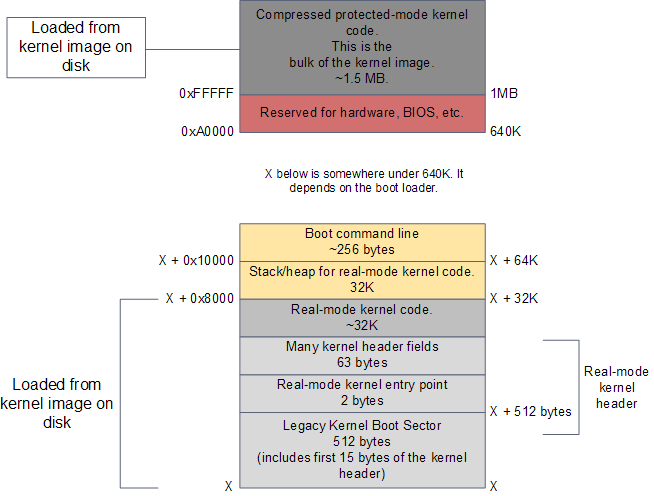
\includegraphics[width=0.5\textwidth]{memboot.png}
    \fig{1}{0 pt}{Memory after bootloader \cite{duarte_kern_boot}}
}

\iffalse
You can startup the kernel in various modes: either protected, real etc. Kernel Boot Protocol: tells the OS how is it going to startup it. Assume that the bootloader stage 1 and stage 2 startup the kernel in real mode. 
\fi

\section{Kernel Initialization}

The bootloader ensures that the kernel is loaded as shown in Figure 4.1 with the Real-mode kernel loaded in the first megabyte of memory and the compressed Protected-mode image right after the first megabyte of memory \footnote{The loading above the first megabyte is performed either through BIOS facilities or Unreal Mode. Remember that the bootloader as well runs in Real-mode first therefore it cannot access that region of memory directly}. After loading the kernel, it jumps to the
\texttt{_start} label placed at 512 bytes of offset from the address where the first Real-mode sector was loaded. From now on is the kernel that will execute in Real-mode.

The first instruction performed is an hardcoded instruction opcode 16-bit short jump \footnote{
The jump is hardcoded to prevent the compiler from producing 32-bit code (instead of 16-bit) where such instruction has a 3 byte opcode. The instruction takes as input an immediate and will set the instruction pointer to the address of the instruction following the jump plus the immediate passed as input. The immediate is computed at compile time through the gnu assembler functionalities where \texttt{start_of_setup} is the label corresponding to the address where the kernel has to jump to and \texttt{1f}
is the label \texttt{1} forward (\texttt{f}) which corresponds to the value of the instruction pointer when the jump instruction will be evaluated.}

to skip the second part of the header and execute code at \texttt{start_of_setup}.

\begin{verbatim}
> arch/x86/boot/header.S
    _start:
        .byte 0xeb
        .byte start_of_setup-1f
    1:
\end{verbatim}

The \texttt{start_of_setup} routine \marginnote{\textsc{Start Of Setup}} first ensures \texttt{\%es = \%ds} so it is possible to use the two segment registers interchangeably and sets  \marginpar{\texttt{\hspace*{1cm} pushw \%ds} \\ \texttt{\hspace*{1cm} pushw 6f,} \\\texttt{\hspace*{1cm} lret}  \\\texttt{6:}} the \texttt{\%cs} register to the same value of the other segment registers through the code shown on the left which sets \texttt{\%cs} to the value written on the stack above the return address and jumps to the label following. 

After that \marginnote{\cite{linin}} it setups a preliminary stack and zeroes the \texttt{.bss} section that holds the unitialized variables since a malevolent or buggy bootloader might have changed some of them.

Finally it jumps to the \texttt{main()} function found in \texttt{arch/x86/boot/main.c}

In the \texttt{main} function \marginnote{\textsc{Boot Main}} the following initializations are performed.


\begin{verbatim}
> arch/x86/boot/main.c

main(void)
    copy_boot_params(void)
        copies the parameters of the Kernel header into a struct

    console_init(void)
        initializes console for printing on screen or serial
        communication

    init_heap(void)
        initializes a heap

    check_cpu(void)
        discovers cpu features

    detect_memory(void)
        invokes the E820 BIOS facility for generating the physical
        memory map

    // other initialization ...

    go_to_protected_mode(void)
        switches to Protected Mode
\end{verbatim}

The \texttt{go_to_protected_mode()} function \marginnote{\textsc{Go To Protected Mode}} performs the last preparations before entering Protected Mode and finally executes Protected-mode code.

\begin{verbatim}
> arch/x86/boot/pm.c

go_to_protected_mode(void)

    realmode_switch_hook(void)
        disable Non Maskable Interrupts (NMI)

    enable_a20(void)
        enable A20 Line as shown in previous lectures

    mask_all_interrupts(void)

    setup_idt(void) {
            static const struct gdt_ptr null_idt = {0, 0};
            asm volatile("lidtl %0" : : "m" (null_idt));
        }
        
        setups a dummy IDT
\end{verbatim}

\marginnote{ The IDT and GDT are initialized at this stage because otherwise the processor won't enter in Protected mode as shown in the
    \href{https://github.com/torvalds/linux/commit/88089519f302f1296b4739be45699f06f728ec31}{commit message}
}[-2.7cm]

\begin{verbatim}
    setup_gdt(void) {
            static const u64 boot_gdt[] __attribute__((aligned(16))) = {
                [GDT_ENTRY_BOOT_CS] = GDT_ENTRY(0xc09b, 0, 0xfffff),
                [GDT_ENTRY_BOOT_DS] = GDT_ENTRY(0xc093, 0, 0xfffff),
                [GDT_ENTRY_BOOT_TSS] = GDT_ENTRY(0x0089, 4096, 103),
            };

            static struct gdt_ptr gdt;
            gdt.len = sizeof(boot_gdt)-1;
            gdt.ptr = (u32)&boot_gdt + (ds() << 4);

            asm volatile("lgdtl %0" : : "m" (gdt));
        }

    protected_mode_jump(boot_params.hdr.code32_start,
                        (u32)&boot_params + (ds() << 4));
\end{verbatim}

\marginnote{\texttt{GDT_ENTRY} takes in input flags, base and limit of a descriptor and generates the entry. Limit is 4KB $\times (2^{20} - 1) \approx 4$GB (G bit set to 1 through flags)}[-6cm]

The GDT entries indices \texttt{GDT_ENTRY_BOOT_CS}, \texttt{GDT_ENTRY_BOOT_DS}, \texttt{GDT_ENTRY_BOOT_TSS} are respectively 2, 3, 4. Entry 0 is reserved as shown in the Intel documentation \cite{intel} while entry 1 is not used by Linux.



The GDT \texttt{len} must be an unsigned short integer that summed with \texttt{ptr} tells the last byte addressable of the table (that's why 1 is subtracted to it) while the \texttt{ptr} must be the 32 bit physical address (that's why \texttt{gdt.ptr = \&boot_gdt + (\%ds} $\times$ 16) of the 16 byte-aligned memory containing the GDT.


Both the GDT and IDT setup functions use inline assembly to perform hardware specific operations which are respectively to load the GDT register and the IDT register with the content of the memory referenced by \texttt{gdt/null_idt}. In the next paragraph we'll describe more deeply the syntax. 

Finally the routine \texttt{protected_mode_jump(u32 entrypoint, u32 bootparams)} defined in \\ \texttt{arch/x86/boot/pmjump.S} performs the jump to Protected Mode code in \texttt{startup_32}. \marginnote{\textsc{Protected Mode Jump}}[-12pt]

\begin{verbatim}
> arch/x86/boot/pmjump.S

protected_mode_jump(u32 entrypoint, u32 bootparams)
    .code16                 ; tell compiler to produce 16bit opcode 
    ; store bootparams in %esi
    ; calculate pm32 physical address and keep in in 2f

    movw $__BOOT_DS, %cx
    movw $__BOOT_TSS, %di

    movl %cr0, %edx         ; enable protected mode
    orb $X86_CR0_PE, %dl    ; through CR0
    movl %edx, %cr0

    .byte   0x66, 0xea      ; 32-bit ljmp opcode
2:
    .long   in_pm32			
    .word   __BOOT_CS

    .code32                 ; tell compiler to produce 32bit opcode

in_pm32:
    
    ; initialize segment registers
    ; setup stack for debugging
    ; setup Task Register otherwise cannot enable Protected-mode
    ; clear general purpose registers
    ; load Local Descriptor Table otherwise cannot enable Protected-mode
    ; jump to 32-bit entry point startup_32 in
    ;       arch/x86/boot/compressed/head_64.S
\end{verbatim}

As the reader may have noticed the code to which the previous snippet jumps to belongs to the \texttt{compressed/} folder under the \texttt{arch/x86/boot/} directory. This is the entry point of the kernel in case of booting through EFI.


Also notice that the code that we are going to explore is for the \texttt{x86_64} architecture. The flow is similar for \texttt{x86_32} and the code can be found in the same folder in \texttt{head_32.S}

The first instruction \marginnote{\textsc{Startup 32 | Compressed} \\ Note that the initialization shown in class is about the \texttt{x86_32} kernel following the code in \texttt{head_32.S} and described in the previous lecture} performed is \texttt{cld} which clears DF used by \texttt{stos} and \texttt{scas} instructions. Then a test on the \texttt{KEEP_SEGMENTS} parameter in the headers set by the bootloader is performed to check whether to reinitialize the segment registers.

In order to know the current physical address where the kernel was loaded the following instructions are performed

\begin{verbatim}
> arch/x86/boot/compressed/head_64.S

    leal    (BP_scratch+4)(%esi), %esp
    call    1f
1:  popl    %ebp
    subl    $1b, %ebp

\end{verbatim}

The stack pointer is set to a physical address known to be "scratchable" to perform the instructions. A \texttt{call} to the following instruction is issued which pushes in the stack the value of the current address of execution which is then \texttt{pop}ped in the \texttt{\%ebp} register. To this value is subtracted the relative address (with respect to the start of the binary object) of label \texttt{1} getting the physical address of \texttt{startup_32}.

Next, knowing the physical address, a stack is setup, a cpu verification is performed to know whether the architecture provides long mode and calculates the relocation address (physical address where the kernel will be loaded).

The last operations are preparations for entering long mode. A new GDT is setup since the previous ones were set for only 32-bit mode (different L and D flags from these ones). The PAE bit is set in \texttt{\%cr4} and an early page table initialization is performed and its address set into \texttt{\%cr3}.

Finally long mode is enabled through the EFER model specific register as shown in the previous lectures, the address of the next routine to be executed is pushed in the stack, paging is enabled by setting the PG bit and the PE bit in \texttt{\%cr0} and \texttt{lret} instruction is issued to start execute \texttt{startup_64} still in \texttt{head_64.S}. In \texttt{startup_64} the bss section is cleared to prepare for the jump to the C code of \texttt{extract_kernel()}
(arch/x86/boot/compressed/misc.c) which will decompress
the kernel and set \texttt{\%rax} to the address at which the kernel was decompressed. \texttt{head_64.S} then jumps to it with \texttt{jmp *\%rax}. 

The kernel \marginnote{\textsc{Startup 64 | Kernel}} entry point is \texttt{startup_64} which code is in \texttt{arch/x86/kernel/head_64.S} (similarly there are two files for the \texttt{x86_32} kernel) that modifies slightly the page table and jumps to \texttt{x86_64_start_kernel()} defined in \texttt{arch/x86/kernel/head64.c} which finally calls \texttt{start_kernel()} defined in \texttt{init/main.c}. \texttt{start_kernel()} will perform many kinds of
system initializations and wake up the other cores through the INIT-SIPI signals.

\iffalse
Steady state is the final state of the system. The kernel must know which core it is running on.  A function in the kernel is implemented to know it. SMP processor id: symmetric multicore processing. Two main ways to know it are through the usage of APIC since the LAPIC holds info telling which LAPIC is answering, or on older version through specific instructions for example cpuid to know cache levels, amd or intel etc. Throws out every kind of information. Paging etc.
\fi

\section{Inline Assembly}

Inline Assembly is a feature provided by the GNU compiler and adopted by other compilers to embed assembly instructions inside C/C++ code. Such construct is useful when some code needs to be highly efficient and even writing it as an asm function (\texttt{fun.S}) the \texttt{call} overhead would be too much or implementing highly hardware-specific code. Both cases suggest that a lot of kernel code contains inline assembly.

The syntax for using inline assembly is:
\begin{verbatim}
asm [volatile] ( AssemblerTemplate 
                 [ : OutputOperands ]
                 [ : InputOperands  ]
                 [ : Clobbers       ] )
\end{verbatim}

Both the \texttt{asm} and \texttt{volatile} keywords can be used with or without underscores (e.g. \texttt{__asm__}). The \texttt{volatile} keyword prevents the assembler from optimizing this portion of code by either removing it or placing it into other positions. It does \textit{not} ensure the ordering of the instructions between assembly and C code.

An example of inline assembly is the following: \texttt{asm ("movl \%\%eax, \%\%ebx");}.

When referring to registers two \% symbols are needed since the usage of just one \% symbol is reserved for referring to C variables inside the Assembler Template. To refer to C variables in the inline assembly code we must "define" them inside the Input or Output operands. The Clobber part informs the compiler what registers or memory areas are going to be modified since it does not parse the assembler template.

Let's look at some examples to get a better idea.
\begin{verbatim}
void cpuid(int code, uint32_t *a, uint32_t *d) {
    asm volatile("cpuid"
        :"=a"(*a),"=d"(*d)
        :"a"(code)
        :"ecx","ebx");
} 
\end{verbatim}

The code above performs the \texttt{cpuid} instruction. The \texttt{code} variable is stored int the \texttt{\%eax} register before issuing the \texttt{cpuid} instruction through the input operands and the contents in the \texttt{\%eax} (\texttt{a}) register and \texttt{\%edx} (\texttt{d}) register are respectively written (\texttt{=}) in the memory area pointed by the variable \texttt{a} (\texttt{(*a)}) and \texttt{d} (\texttt{(*d)}) after the instruction.
Indeed if we compile the code above we get:

\begin{verbatim}
cpuid(int, int*, int*):
    pushl %ebx
    movl 8(%esp), %eax      ; a (code)
    cpuid
    movl 12(%esp), %ecx     ;
    movl %eax, (%ecx)       ; =a (*a)
    movl 16(%esp), %eax     ;
    movl %edx, (%eax)       ; =d (*d)
    popl %ebx
    ret 
\end{verbatim}

Another example is the \texttt{swap} function below.

\begin{verbatim}
void swap(long *a, long *b){
    __asm__ __volatile__ (
        "push (%%rax) \n"
        "push (%%rbx) \n"
        "pop (%%rax)  \n"
        "pop (%%rbx)"
        : 	"=a" (a) , "=b" (b)
        :	"0" (a) , "1" (b)
        :	"memory"
    );
} 
\end{verbatim}

The variables passed as input are moved to the \texttt{rax} and \texttt{rbx} registers and the values stored in the memory pointed by the two pointers are pushed to then be popped in the reverse order into the memory pointed by the two pointers. In the input operands the registers are referred through the sequential enumeration offered by GCC. With string \texttt{"0"} it refers to the 0th register declared in the output/input operands, i.e. \texttt{\%rax} in this case, while string \texttt{"1"}
refers to the 1st register declared which is \texttt{\%rbx}.

Setting the string \texttt{"memory"} into the clobbers informs the compiler that the portion of inline assembly performs side effect in memory and ensures that the compiler won't perform any kind of reordering in the scope in which the inline assembly is written.

Last example

\begin{verbatim}
bool CAS(volatile unsigned long long *ptr,
        unsigned long long oldVal,
        unsigned long long newVal) {
    unsigned long res = 0;

    __asm__ __volatile__(
        "lock cmpxchgq %1, %2;"//ZF = 1 if succeeded
        "lahf;"         // to get the correct result even if oldVal == 0
        "bt $14, %%ax;" // is ZF set? (ZF is the 6'th bit in %ah,
                        // so it's the 14'th in ax)
        "adc %0, %0"    // get the result
        : "=r"(res)
        : "r"(newVal), "m"(*ptr), "a"(oldVal), "0"(res)
        : "memory"
	);

    return (bool) res;
}
\end{verbatim}

The code produced by the assembler is the following

\begin{verbatim}
CAS(unsigned long long volatile*, unsigned long long, unsigned long long):
    xorl %ecx, %ecx
    movq %rsi, %rax
    lock cmpxchgq %rdx, (%rdi);
    lahf;
    bt $14, %ax 
    adc %rcx, %rcx
    testq %rcx, %rcx
    setne %al
    ret
\end{verbatim}

From the \texttt{x64} calling convention the first three parameters are stored into registers \texttt{\%rdi, \%rsi, \%rdx}. \texttt{oldVal} which is in \texttt{\%rsi} is moved into \texttt{\%rax} as required by the input operand. In the inline assembly \texttt{cmpxchgq} takes in input the 1st and 2nd input operands which are \texttt{newVal} and \texttt{ptr} that are stored \texttt{\%rdx} and \texttt{\%rdi}.

\subsection{Kernel Initialization Signature}

Another important fact to be analyzed is the \texttt{start_kernel()} signature which has the following macros prepended to it:

\begin{description}
    \item \texttt{asmlinkage}: in order to be more performant in i386 architecture the kernel is compiled with the option \texttt{-mregparm=3} which forces GCC to optimize function calls by putting the parameters into the registers instead of putting them on stack as defined by the ABI. This macro ensures that the parameters passed to the function will be on stack. 
    \item \texttt{__visible}: informs the compiler to not remove the function during the link-time optimization even if it is not called by any code
    \item \texttt{__init}: sets the function binary into a specific region of memory called \texttt{.init.text} allowing the kernel to safely reclaim that space after initialization is concluded
\end{description}

\newpage
\bibliography{Lec4}
\bibliographystyle{plainnat}
\end{document}
